\documentclass[10pt]{article}
\usepackage[letterpaper]{geometry}
\geometry{verbose,tmargin=1in,bmargin=1in,lmargin=1in,rmargin=1in}
\usepackage{setspace}
\usepackage{ragged2e}
\usepackage{color}
\usepackage{titlesec}
\usepackage{graphicx}
\usepackage{float}
\usepackage{mathtools}
\usepackage{amsmath}
\usepackage[font=small,labelfont=bf,labelsep=period]{caption}
\usepackage[english]{babel}
\usepackage{indentfirst}
\usepackage{array}
\usepackage{makecell}
\usepackage[usenames,dvipsnames]{xcolor}
\usepackage{multirow}
\usepackage{tabularx}
\usepackage{arydshln}
\usepackage{caption}
\usepackage{subcaption}
\usepackage{xfrac}
\usepackage{etoolbox}
\usepackage{cite}
\usepackage{url}
\usepackage{dcolumn}
\usepackage{hyperref}
\usepackage{courier}
\usepackage{esvect}
\usepackage{commath}
\usepackage{verbatim} % for block comments
\usepackage{enumitem}
\usepackage{hyperref} % for clickable table of contents
\usepackage{braket}
\usepackage{titlesec}
\usepackage{booktabs}
\usepackage{gensymb}
\usepackage{listings}
\usepackage{cancel}
\usepackage[mathscr]{euscript}
\lstset{
    frame=single,
    	basicstyle=\ttfamily\small,
    breaklines=true,
    postbreak=\raisebox{0ex}[0ex][0ex]{\ensuremath{\color{red}\hookrightarrow\space}}
}

% for circled numbers
\usepackage{tikz}
\newcommand*\circled[1]{\tikz[baseline=(char.base)]{
            \node[shape=circle,draw,inner sep=2pt] (char) {#1};}}

\newcommand{\beq}{\begin{equation}}
\newcommand{\eeq}{\end{equation}}
\newcommand{\beqa}{\begin{equation}\begin{aligned}}
\newcommand{\eeqa}{\end{aligned}\end{equation}}

\titleclass{\subsubsubsection}{straight}[\subsection]

% define new command for triple sub sections
\newcounter{subsubsubsection}[subsubsection]
\renewcommand\thesubsubsubsection{\thesubsubsection.\arabic{subsubsubsection}}
\renewcommand\theparagraph{\thesubsubsubsection.\arabic{paragraph}} % optional; useful if paragraphs are to be numbered

\titleformat{\subsubsubsection}
  {\normalfont\normalsize\bfseries}{\thesubsubsubsection}{1em}{}
\titlespacing*{\subsubsubsection}
{0pt}{3.25ex plus 1ex minus .2ex}{1.5ex plus .2ex}

\makeatletter
\renewcommand\paragraph{\@startsection{paragraph}{5}{\z@}%
  {3.25ex \@plus1ex \@minus.2ex}%
  {-1em}%
  {\normalfont\normalsize\bfseries}}
\renewcommand\subparagraph{\@startsection{subparagraph}{6}{\parindent}%
  {3.25ex \@plus1ex \@minus .2ex}%
  {-1em}%
  {\normalfont\normalsize\bfseries}}
\def\toclevel@subsubsubsection{4}
\def\toclevel@paragraph{5}
\def\toclevel@paragraph{6}
\def\l@subsubsubsection{\@dottedtocline{4}{7em}{4em}}
\def\l@paragraph{\@dottedtocline{5}{10em}{5em}}
\def\l@subparagraph{\@dottedtocline{6}{14em}{6em}}
\makeatother

\newcommand{\volume}{\mathop{\ooalign{\hfil$V$\hfil\cr\kern0.08em--\hfil\cr}}\nolimits}

\setcounter{secnumdepth}{4}
\setcounter{tocdepth}{4}
\begin{document}

\title{MATH 228b: HW5... 2ab}
\author{April Novak}

\maketitle

\section{}

The first part of this question requires replacing equidistant node positions with the Chebyshev nodes, which should eliminate Runge phenomena, which is commonly observed as oscillations in high-degree polynomials. The Chebyshev node positions \(s_i\) are given as \(s_i=\cos{(\pi i/p)}\), where \(p=0, \cdots, P\), where \(P\) is the polynomial order of the shape functions. The Chebyshev nodes are defined on \([-1, 1]\), so to transform these to a single element defined over \([0, h]\), the Chebyshev nodes are multiplied by \(-2/h\), where 2 is the length of the domain of the Chebyshev nodes, and \(h\) the length of the desired domain.

Next, we need to compute the elementary mass and stiffness matrices. The strong form of the governing equation is:

\beqa
\frac{\partial u}{\partial t}+\frac{\partial u}{\partial x}=&0\\
\frac{\partial u}{\partial t}+\frac{\partial f(u)}{\partial x}=&0\\
\eeqa

where \(f(u)=u\) is the flux function. We will expand the solution \(u\) in a single element:

\beq
u_h=\sum_{j=0}^{P}u_j\phi_j
\eeq

and over the entire domain of \(K\) elements:

\beq
u_h=\sum_{k=1}^{K}\sum_{j=0}^{P}u_j^k\phi_j^k(x)
\eeq

where \(\phi_j\) are the expansion functions within a single element. Following the Galerkin approach, the test function \(v_h\) will also be expanded in the same set of basis functions. Integrate the flux term by parts, which due to the discontinuous nature of \(u_h\) and \(v_h\) cannot technically be performed. It is here that the discontinuous Galerkin method borrow from the finite volume method. For the discontinuities, approximate using a numerical flux function \(F(u_h)\). At the left side of an element (at \(x_{k}\)), this numerical flux should depend (at a minimum at least) only on \(u_0^k\) and \(u_P^{k-1}\), where now a new notation is introduced to describe the multiple expansion coefficients in each element (ranging from 0 to \(P\)). 

\beqa
\int_{\Omega}\frac{\partial u_h}{\partial t}v_hdx+\int_{\Omega}\frac{\partial f(u_h)}{\partial x}v_hdx=&0\\
\int_{\Omega}\frac{\partial u_h}{\partial t}v_hdx-\int_{\Omega}f(u_h)\frac{\partial v_h}{\partial x}dx+\left\lbrack f(u_h)v_h\cdot\hat{n}\right\rbrack_{x_{k-i}}^{x_k}=&0\\
\int_{\Omega}\frac{\partial u_h}{\partial t}v_hdx-\int_{\Omega}f(u_h)\frac{\partial v_h}{\partial x}dx+F(u_0^{k+1}, u_P^k)v_h(x_{k})-F(u_0^k, u_P^{k-1})v_h(x_{k-1})=&0\\
\eeqa

Substituting in the expansion over a single element into the equation above:

\beqa
\int_{\Omega}\frac{\partial}{\partial t}\left(\sum_{j=0}^{P}u_j\phi_j(x)\right)\sum_{i=0}^{P}v_i\phi_i(x)dx-\int_{\Omega}f(u_h)\frac{\partial}{\partial x}\left(\sum_{i=0}^{P}v_i\phi_i(x)\right)dx+\quad\\
F(u_0^{k+1}, u_P^k)\sum_{i=0}^{P}v_i\phi_i(x_{k})-F(u_0^k, u_P^{k-1})\sum_{i=0}^{P}v_i\phi_i(x_{k-1})=0\\
\eeqa

Then, because \(v_i\) appears in every term and is arbitrary, it can be ``cancelled'' from each term by pulling the summation over \(i\) outside all integrals such that the integrand must be zero.

\beqa
\int_{\Omega}\frac{\partial}{\partial t}\left(\sum_{j=0}^{P}u_j\phi_j(x)\right)\sum_{i=0}^{P}\phi_i(x)dx-\int_{\Omega}f(u_h)\frac{\partial}{\partial x}\left(\sum_{i=0}^{P}\phi_i(x)\right)dx+\quad\\
F(u_0^{k+1}, u_P^k)\sum_{i=0}^{P}\phi_i(x_{k})-F(u_0^k, u_P^{k-1})\sum_{i=0}^{P}\phi_i(x_{k-1})=0\\
\eeqa

Then, while the above equation is true, it is also true that it holds for each individual choice of \(i\) and \(j\) such that the summations can be removed with the implicit assumption of creating matrices that are of size \(p+1\times p+1\) for the creation of a system of equations that holds for a single element. For the case of linear advection, \(f(u_h)=u_h\), giving the second form below.

\beqa
\int_{\Omega}\frac{\partial u_j}{\partial t}\phi_j(x)\phi_i(x)dx-\int_{\Omega}f(u_h)\frac{\partial \phi_i(x)}{\partial x}dx+F(u_0^{k+1}, u_P^k)\phi_i(x_{k})-F(u_0^k, u_P^{k-1})\phi_i(x_{k-1})=&0\\
\int_{\Omega}\frac{\partial u_j}{\partial t}\phi_j(x)\phi_i(x)dx-\int_{\Omega}u_j\phi_j(x)\frac{\partial \phi_i(x)}{\partial x}dx+F(u_0^{k+1}, u_P^k)\phi_i(x_{k})-F(u_0^k, u_P^{k-1})\phi_i(x_{k-1})=&0\\
\eeqa

Define the mass matrix \(M_{ij}\) as:

\beq
M_{ij}^k=\int_{x_{k-1}}^{x_k}\phi_j(x)\phi_i(x)dx
\eeq

and the stiffness matrix \(K_{ij}^k\) as:

\beq
K_{ij}^k=\int_{x_{k-1}}^{x_k}\phi_j(x)\frac{\partial \phi_i(x)}{\partial x}dx
\eeq

For linear advection (i.e. with constant velocity), a good choice of numerical flux is to use upwinding such that the downwind value is always selected as the numerical flux. Then, the weak form becomes:

\beq
\int_{\Omega}\frac{\partial u_j}{\partial t}\phi_j(x)\phi_i(x)dx-\int_{\Omega}u_j\phi_j(x)\frac{\partial \phi_i(x)}{\partial x}dx+u_P^k\phi_i^k(x_{k})-u_P^{k-1}\phi_i^k(x_{k-1})=0\\
\eeq

Then a system of equations that holds for a single element is:

\beq
M_{ij}^k\dot{u_j}^k-K_{ij}^ku_j^k+u_P^k\phi_i^k(x_{k})-u_P^{k-1}\phi_i^k(x_{k-1})=0
\eeq

Because we will use nodal basis functions, \(\phi_i^k(x_k)\) and \(\phi_i^k(x_{k-1})\) are zero at all nodes except a single node. Hence, all of these extra terms will drop out except for one term each, and the shape function at that node will be unity.

Finally, to implement arbitrary order polynomials, the mass and stiffness matrices must be computed. Because very high order polynomials will be used, these should be computed in a domain over \([-1,1]\) so that Gaussian quadrature can easily be used. These matrices transform according to:

\beqa
M_{ij}^k=&\int_{-1}^{1}\phi_j(\xi)\phi_i(\xi)\frac{dx}{d\xi}d\xi\\
=&\int_{-1}^{1}\phi_j(\xi)\phi_i(\xi)\frac{h}{2}d\xi\\
\eeqa

where \(-1\leq\xi\leq1\) represents the domain over which the integration will occur and the Jacobian of the transformation in 1-D is simply \(h/2\) because the length of the domain in the physical domain is \(h\) and the length in the \(\xi\) domain is 2. Likewise, the stiffness matrix transforms according to:

\beqa
K_{ij}^k=&\int_{-1}^{1}\phi_j(\xi)\frac{\partial \phi_i(\xi)}{\partial \xi}\frac{\partial \xi}{\partial x}\frac{\partial x}{\partial \xi}d\xi\\
=&\int_{-1}^{1}\phi_j(\xi)\frac{\partial \phi_i(\xi)}{\partial \xi}d\xi\\
\eeqa

Legendre polynomials are used as the expansion functions for this problem because they will eliminate the oscillatory nature of higher-degree monomials. However, the stand-alone Legendre polynomials are not a nodal basis. To make these polynomials a nodal basis, we write our basis functions \(\phi_i\) as a sum of \(P\) Legendre polynomials:

\beq
\phi_i(\xi)=\sum_{i=0}^Pc_i^jP_j(\xi)
\eeq

For \(P=2\) (just for example), the coefficients \(c_i^j\) can be determined by requiring that the basis function goes to zero at all nodes except one. For nodes \(s_p\) (of which there are \(p+1\)):

\beq
\begin{bmatrix}
P_0(s_0) & P_1(s_0) & P_2(s_0)\\
P_0(s_1) & P_1(s_1) & P_2(s_1)\\
P_0(s_2) & P_1(s_2) & P_2(s_2)\\
\end{bmatrix}
\begin{bmatrix}
c_0^0 & c_1^0 & c_2^0\\
c_0^1 & c_1^1 & c_2^1\\
c_0^2 & c_1^2 & c_2^2\\
\end{bmatrix}=
\begin{bmatrix}
1 & 0 & 0\\
0 & 1 & 0\\
0 & 0 & 1
\end{bmatrix}
\eeq

This must be performed for each element to determine the basis functions for each element. Alternatively, because the integrals are to be performed in the \(\xi\) domain anyways, these can be found a single time in the \(\xi\) domain (and then reused for every element). After these coefficients are determined, the elemental mass and stiffness matrices are determined according to the equations given previously. The {\tt legendre\_poly.m} function is used for evaluating these polynomials and their derivatives over the reference element. Then, the remainder of the solve does not need to be modified, since at this point it is a ``turn-the-crank'' procedure.

To plot the solution using \(3P\) points per element requires using the nodal values to determine the solution in each element. We need to evaluate the solution at these points in order to be able to interpolate the solution values at these \(3P\) points with straight lines (as requested). Because all of the integrals were transformed to the reference element appropriately, all of the solution values {\tt u} obtained during the time-stepping loop are valid in the physical domain. However, for plotting, the expansion functions in the physical domain must be determined - up until now, they have only been defined for a reference element. The solution over an element in the reference domain for \(P=2\) is:

\beq
u_h^{e=1}=C_1^0\phi_0(\xi)+C_1^1\phi_1(\xi)+C_1^2\phi_2(\xi)
\eeq

And in the physical domain, it is:

\beq
u_h^{e=1}=u_1^0\phi_0(x)+u_1^1\phi_1(x)+u_1^2\phi_2(x)
\eeq

But, the expansion functions are only known in the reference element. Because the Legendre polynomials form a basis, we can express any \(P\)-order polynomial using a summation of \(P\) Legendre polynomials. Hence, for \(P=2\) for instance, the solution in each element is a cubic of the form:

\beq
u_h^e=A_0^e+A_1^ex+A_2^ex^2
\eeq

where once these coefficients are determined, the solution over the element is fully known. For an element \(e=1\) with nodes at \(x=0.25, 0.5, 0.75\), we can solve for these coefficients \(A\) by:

\beq
\begin{bmatrix}
1\cdot 0.25^0 & 1\cdot 0.25^1 & 1\cdot 0.25^2\\
1\cdot 0.50^0 & 1\cdot 0.50^1 & 1\cdot 0.50^2\\
1\cdot 0.75^0 & 1\cdot 0.75^1 & 1\cdot 0.75^2
\end{bmatrix}
\begin{bmatrix}
A_0^1\\
A_1^1\\
A_2^1
\end{bmatrix}
=
\begin{bmatrix}
u_1^0\\
u_1^1\\
u_1^2
\end{bmatrix}
\eeq

This is then repeated for every element until the solution over each element is fully specified. Then, the monomial defined using the coefficients \(A\) is sampled at the desired interpolation points for plotting purposes (at \(3P\) points). 

Finally, to compute the error, the \(L^2\) norm is computed over the entire domain. Because the solution is discontinuous, this is straightforward, and the solution over each element is integrated from \(x_{k-1}\) to \(x_k\) and then summed (and then square-rooted). To compute the norm, the exact solution is interpolated into a discontinuous Galerkin basis (i.e. it is expressed in the same form as {\tt u} from the original {\tt dgconvect0.m} code), and then trapezoidal integration is performed over each element by simply taking the square of the difference entry-wise between the discontinuous Galerkin solution and the analytical solution. To ensure that accurate norms are obtained, the interpolation of the analytical and numerical solutions into new spatial domains of length 500 nodes/element is performed. Because the error can be found at each time step, for comparison it is only evaluated and compared for the last time step.

The {\tt errors} matrix returned by {\tt dgconvect\_convergence} reports errors in the format such that each row corresponds to the errors for a given \(p\). Fig. \ref{fig:errors_raw} shows the raw data obtained for the requested points (and more to obtain better slope estimates) for all five of the polynomial orders. As can be seen, points below a logarithm of the \(L^2\) norm of about \(10^{-8}\) are affected by numerical rounding, since theoretically the error should monotonically decrease. Fig. \ref{fig:errors} shows the same data, but with points with an \(L^2\) norm less that \(10^{-8}\) removed from the data set. As can be seen, once these spurious data points are removed, all polynomial orders except 16 obtain fairly close to theoretical convergence rates. Like the continuous Galerkin method, the rate of convergence in the \(L^2\) norm should be the order of the polynomial expansion plus one. A poor rate of convergence is observed for \(p=16\) (and somewhat also for \(p=8\), which converges at a slope less than theoretical) because at such a fine solution, the time error associated with the Runge-Kutta stepping likely dominates the total error. To completely eliminate the time error, a method of manufactured solutions test could be performed to show that for an analytical, \textit{linear}, dependence on time, all of the polynomial orders should obtain theoretical convergences. All  of the code for this section is included in the Appendix. For the purpose of replicating these convergence results, the plotting section of {\tt dgconvect} should be commented out.

\begin{figure}[H]
\centering
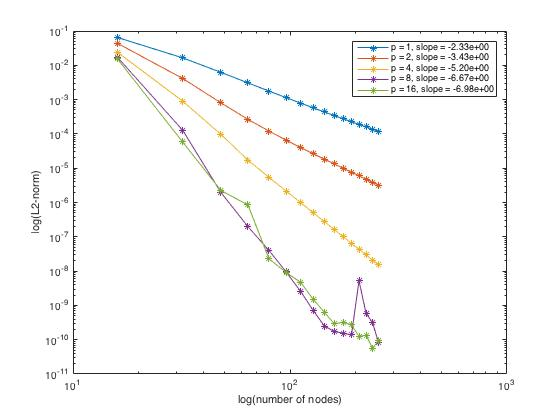
\includegraphics[width=0.8\textwidth]{figures/errors_raw.jpg}
\caption{\(L^2\) norm as a function of the number of nodes.}
\label{fig:errors_raw}
\end{figure}

\begin{figure}[H]
\centering
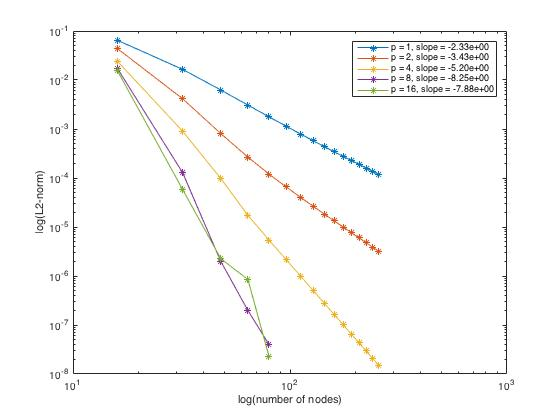
\includegraphics[width=0.8\textwidth]{figures/errors.jpg}
\caption{\(L^2\) norm as a function of the number of nodes with data points with an \(L^2\) norm less that \(10^{-9}\) removed from the data.}
\label{fig:errors}
\end{figure}






\section{}

This problem modifies the code developed in the first part by solving the convection-diffusion equation:

\beq
\frac{\partial u}{\partial t}+\frac{\partial f(u)}{\partial x}-k\frac{\partial^2 u}{\partial x^2}=0
\eeq

The solution approach follows that in question 1, where again \(f(u)=u\), except that the above will be split into a system of two first-order equations, because otherwise we would need to determine a numerical ``flux function'' for specifying \(\partial u/\partial x\) on the boundary, which can be difficult.

\beqa
\frac{\partial u}{\partial t}+\frac{\partial f(u)}{\partial x}-k\frac{\partial \sigma}{\partial x}=0\\
\sigma=\frac{\partial u}{\partial x}\\
\eeqa

Then, the approach from here is similar to that taken in the first problem. Express \(u\) and the test function \(v\) as an expansion, integrate over space, and integrate by parts when possible. The shape function used in the equation for \(\sigma\) is denoted as \(\tau\).

\beqa
\int_{\Omega}\frac{\partial u_h}{\partial t}v_hdx+\int_{\Omega}\frac{\partial f(u_h)}{\partial x}v_hdx-\int_{\Omega}k\frac{\partial \sigma_h}{\partial x}v_h=0\\
\int_{\Omega}\sigma_h\tau_hdx=\int_{\Omega}\frac{\partial u_h}{\partial x}\tau_hdx\\
\eeqa

Now, integrate by parts to give:

\beqa
\int_{\Omega}\frac{\partial u_h}{\partial t}v_hdx-\int_{\Omega}\frac{\partial v_h}{\partial x}f(u_h)dx+\int_{\Omega}k\frac{\partial v_h}{\partial x}\sigma_h+\left\lbrack f(u_h)v_h\cdot\hat{n}\right\rbrack_0^1-\left\lbrack k\sigma_hv_h\cdot\hat{n}\right\rbrack_0^1=0\\
\int_{\Omega}\sigma_h\tau_hdx=-\int_{\Omega}\frac{\partial \tau_h}{\partial x}u_hdx+\left\lbrack u_h\tau_h\cdot\hat{n}\right\rbrack_0^1\\
\eeqa

Next, we assume that \(u_h\), \(v_h\), \(\sigma_h\), and \(\tau_h\) all come from the same space of functions. Inserting these expansions into the above gives, for a single element:

\beqa
\int_{x_{k-1}}^{x_k}\frac{\partial}{\partial t}\left(\sum_{j=0}^{P}u_j\phi_j\right)\sum_{i=0}^{P}v_i\phi_idx-\int_{x_{k-1}}^{x_k}\frac{\partial}{\partial x}\left(\sum_{i=0}^{P}v_i\phi_i\right)\sum_{j=0}^{P}u_j\phi_jdx+\quad\\
\int_{x_{k-1}}^{x_k}k\frac{\partial}{\partial x}\left(\sum_{i=0}^{P}v_i\phi_i\right)\sum_{j=0}^{P}\sigma_j\phi_j+\left\lbrack \sum_{j=0}^{P}u_j\phi_j\sum_{i=0}^{P}v_i\phi_i\cdot\hat{n}\right\rbrack_{x_{k-1}}^{x_k}-\left\lbrack k\sum_{j=0}^{P}\sigma_j\phi_j\sum_{i=0}^{P}v_i\phi_i\cdot\hat{n}\right\rbrack_{x_{k-1}}^{x_k}=0\\
\eeqa

\beq
\int_{x_{k-1}}^{x_k}\sum_{j=0}^{P}\sigma_j\phi_j\sum_{i=0}^{P}\tau_i\phi_idx=-\int_{x_{k-1}}^{x_k}\frac{\partial}{\partial x}\left(\sum_{i=0}^{P}\tau_i\phi_i\right)\sum_{j=0}^{P}u_j\phi_jdx+\left\lbrack \sum_{j=0}^{P}u_j\phi_j\sum_{i=0}^{P}\tau_i\phi_i\cdot\hat{n}\right\rbrack_{x_{k-1}}^{x_k}\\
\eeq

Because \(\tau_i\) is arbitrary, it can be ``cancelled'' from every term in the second equation by grouping all of the terms such that \(\tau_i\) multiplies an integrand. Then, that integrand must be zero, allowing \(\tau_i\) to be cancelled. The same argument applies for \(v_i\). Then, while the equations are true when using the entire summation, it is also true for each individual \(p\). 

\beqa
\int_{x_{k-1}}^{x_k}\frac{\partial}{\partial t}\left(\sum_{j=0}^{P}u_j\phi_j\right)\sum_{i=0}^{P}\phi_idx-\int_{x_{k-1}}^{x_k}\frac{\partial}{\partial x}\left(\sum_{i=0}^{P}\phi_i\right)\sum_{j=0}^{P}u_j\phi_jdx+\quad\\
\int_{x_{k-1}}^{x_k}k\frac{\partial}{\partial x}\left(\sum_{i=0}^{P}\phi_i\right)\sum_{j=0}^{P}\sigma_j\phi_j+\left\lbrack \sum_{j=0}^{P}u_j\phi_j\sum_{i=0}^{P}\phi_i\cdot\hat{n}\right\rbrack_{x_{k-1}}^{x_k}-\left\lbrack k\sum_{j=0}^{P}\sigma_j\phi_j\sum_{i=0}^{P}\phi_i\cdot\hat{n}\right\rbrack_{x_{k-1}}^{x_k}=0\\
\\
\int_{x_{k-1}}^{x_k}\frac{\partial}{\partial t}\left(u_j\phi_j\right)\phi_idx-\int_{x_{k-1}}^{x_k}\frac{\partial\phi_i}{\partial x}u_j\phi_jdx+\quad\\
\int_{x_{k-1}}^{x_k}k\frac{\partial\phi_i}{\partial x}\sigma_j\phi_j+\left\lbrack u_j\phi_j\phi_i\cdot\hat{n}\right\rbrack_{x_{k-1}}^{x_k}-\left\lbrack k\sigma_j\phi_j\phi_i\cdot\hat{n}\right\rbrack_{x_{k-1}}^{x_k}=0\\
\eeqa

\beqa
\int_{x_{k-1}}^{x_k}\sum_{j=0}^{P}\sigma_j\phi_j\sum_{i=0}^{P}\phi_idx=&-\int_{x_{k-1}}^{x_k}\frac{\partial}{\partial x}\left(\sum_{i=0}^{P}\phi_i\right)\sum_{j=0}^{P}u_j\phi_jdx+\left\lbrack \sum_{j=0}^{P}u_j\phi_j\sum_{i=0}^{P}\phi_i\cdot\hat{n}\right\rbrack_{x_{k-1}}^{x_k}\\
\int_{x_{k-1}}^{x_k}\sigma_j\phi_j\phi_idx=&-\int_{x_{k-1}}^{x_k}\frac{\partial\phi_i}{\partial x}u_j\phi_jdx+\left\lbrack u_j\phi_j\phi_i\cdot\hat{n}\right\rbrack_{x_{k-1}}^{x_k}\\
\eeqa

Define a mass matrix as:

\beq
M_{ij}^k=\int_{x_{k-1}}^{x_k}\phi_j\phi_idx
\eeq

and a stiffness matrix as:

\beq
K_{ij}^k=\int_{x_{k-1}}^{x_k}\frac{\partial\phi_i}{\partial x}\phi_jdx
\eeq



Then, the system of equations becomes, for a single element:

\beq
M_{ij}^k\sigma_j^k=-K_{ij}^ku_j^k+\begin{bmatrix}\end{bmatrix}
\eeq



\section{Appendix}
\subsection{Question 1}
\subsubsection{{\tt dgconvect.m}}
\lstinputlisting[language=Matlab]{dgconvect.m}
\subsubsection{{\tt dgconvect\_convergence.m}}
\lstinputlisting[language=Matlab]{dgconvect_convergence.m}


\end{document}
